\chapter{Kravspecifikation}
\label{ch:kravspecikikation}
Kravspecifikationen er udarbejdet i begyndelsen af projektforløbet og omfatter use cases, ikke-funktionelle krav samt kvalitetsfaktorer. For den fulde kravspecifikation henvises der til dokumentionsdokumentet \textit{Kravspecifikation}.

\subsection{Overordnede krav til systemet}
Systemet skal indeholde en til flere sensorer til måling af vandstand i tanke, en sensor eller flere sensorer til måling af skibshældning, en grafisk brugergrænseflade til skibsføreren samt et webinterface til terminalrepræsentanten.

\subsection{Funktionelle krav}
Systemets funktioner er beskrevet ved hjælp af use cases. Før use cases udfærdiges nedskrives systemets aktører. Der udarbejdes en beskrivelse af deres funktion samt ansvar i systemet. Hver use case repræsenterer en enkelt funktionalitet i systemet.
\begin{figure}[H]
\centering
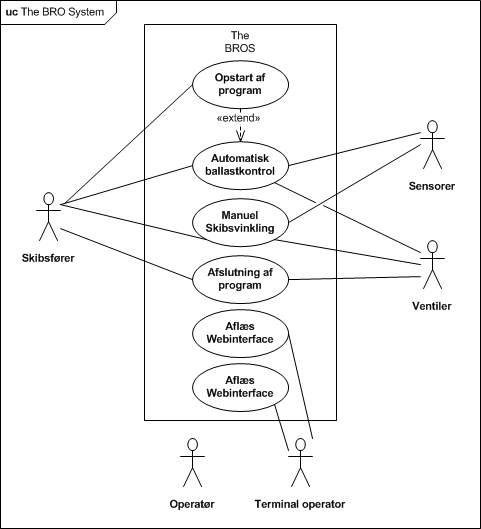
\includegraphics[width=0.4\textwidth]{billeder/UCDBROS}
\caption{Use case diagram for BROS}
\label{fig:UCDBROS}
\end{figure}
Der er også beskrevet alternative hændelser, såfremt hændelsesforløbet ikke forløber som planlagt. Alle use cases har fulgt samme fremgangsprocedure. Se kravspecifikationsdokumentet for alle systemets use cases. På figur \ref{fig:UCDBROS} ses alle use cases for systemet.\\
Når systemet startes op første gang anvendes \textit{Opstart af program} (use case 1). Når systemet er startet op kan brugeren vælge mellem \textit{Automatisk hældningsregulering}(use case 2) eller \textit{Manuel hældningsregulering} (use case 3). Hvis brugeren vil deaktivere systemet kan han afslutte programmet (use case 4). En terminalrepræsentant kan tilgå databaseinformationen via et Webinterface (use case 5 og 6).


\subsection{Ikke-funktionelle krav}
I dette afsnit beskrives krav til tolerancer og andre krav der ikke er use case specifikke. Nedenfor er noteret eksempler på ikke-funktionelle krav:
\begin{itemize}
\item Sensorer:
\begin{itemize}
\item[$\diamond$] Hældningssensor:\\
Hældningssensor måler skibets hældning i forhold til vandret i området -7.5 til 7.5 grader, med en nøjagtighed på $\pm$2.5 grader.\\
\item[$\diamond$] Afstandssensor i ballasttank\\
Vandniveauet i ballasttanken skal måles fra 0-100\% med en nøjagtighed på $\pm$2.5\%-point.
\end{itemize}
\item Alarmer udløses når:
\begin{itemize}
\item[$\diamond$]Vandniveauet i ballasttanke bliver mere end 70\%.
\item[$\diamond$]Hældning på skibet bliver større end $\pm$5 grader.
\item[$\diamond$]Mistet eller ingen forbindelse internt i systemet.
\item[$\diamond$]Mistet eller ingen forbindelse til ekstern database.
\end{itemize}
\end{itemize}
\subsection{Krav til udviklingsprocess og teknologi}
Projektforløbet skal følge V-modellen. Scrum skal bruges i projektstyringsprocessen til at give overblik over projektets arbejdsopgaver. Blandt gruppens medlemmer uddelegeres posterne Scrum-master og projektleder.\\
SysML anvendes til at beskrive systemet overordnet og i detaljer.\\
Til programmeringen af systemets indlejrede enheder anvendes C. Til Kontrolinterfacet og Serveren anvendes C++. Til databaselagring anvendes MySQL. Webinterfacet skal skrives i php og HTML 4.01.

\subsection{Krav til grænseflader}
Kommunikationen mellem Kontrolinterfacet og Styringsmodulet skal følge UART protokollen. Det kan kun tilkobles ét Kontrolinterface og ét Styringsmodul.\\
Til Styringsmodulet tilkobles én sensor samt to Vandballasttankenheder ved hjælp af I2C-protokollen.\\
På kontrolinterfacet skal alt funktionaliteten være indbygget i brugergrænsefladen. Det skal være muligt at skifte mellem automatisk hældningsregulering og manuel hældningsregulering.\\

\subsection{Kvalitetsfaktorer}
For at sikre kvaliteten af produktet er der opstillet en række kvalitetsfaktorer. Det er meget vigtigt at systemet er pålideligt, sikkert og effektivt. Pålideligheden er vigtig da systemet kan risikere at være fatalt for et skib, hvis der sker en fejl. Systemet skal være sikkert da det er et kritisk komponent. Endvidere skal systemet være effektivt da det ikke må sløve lastning- og losningsprocessen.\\
Krav til bruger- og vedligeholdsesvenlighed er middelvægtet, da brugerens anvendelse af systemet skal hjælpe til processen og ikke gøre den yderligere kompliceret. Systemet skal kunne vedligeholdes af en tilkaldt operatør.\\
